\documentclass[12pt]{article}

\usepackage{fullpage,url,amssymb,epsfig,color,pdfpages,xspace,enumerate,multirow,enumitem,graphicx,amsmath}
\usepackage{listings}
\usepackage[pdftitle={ECE457b Project},%
pdfsubject={University of Waterloo, ECE 457b, Winter 2017},%
pdfauthor={Daniel Cardoza, Lara Janecka, Hong Wang}]{hyperref}

\begin{document}

\begin{center}
{\Large\bf Report for}\\
\vspace{1mm}
{\Large\bf ECE457B Course Project, Winter 2017}\\
\vspace{2mm}
{\Large\bf Ultimate DR}\\
\vspace{4mm}
{Daniel Cardoza/dpmcardo/20471664}\\
{Lara Janecka/lajaneck/20460089}\\
{Hong Wang/hmwang/20469058}\\
\vspace{2mm}
\textbf{Due Date: April 3, 2017}
\end{center}

\definecolor{care}{rgb}{0,0,0}
\def\question#1{\item[\bf #1.]}
\def\part#1{\item[\bf #1)]}
\newcommand{\pc}[1]{\mbox{\textbf{#1}}} % pseudocode

\section{Abstract}
\subsection{Introduction}
The project proposed by the following abstract falls underneath Cluster 2 of the possible projects, \textbf{Pattern Recognition and
Perception}. The goal of Ultimate DR is to produce software that is able to generate Dance Dance Revolution (DDR) game
files using neural networks and fuzzy inferencing techniques.
DDR is a video game under the genre of rhythm games. In the game,
the player is presented with music and a sequence of arrows which they must press at an exact
time. Typically, the game is played on a foot-pad where the player presses 4 arrows with their
feet, which is akin to dancing to the music. Currently, DDR game files (SM files) are generated
manually by semi-professional or professional step makers. The step makers create the SM files
by listening to the song and creatively conjuring a set of steps to match the music; the better
the game steps matches the music, the more exciting the song is to play.


\subsection{Motivation}
The main problem with DDR as a game is the lack of SM files for a wide selection of songs. This
is due to the fact that to generate each SM file, a step maker will need to spend around 4 hours.
As the current demand for the game is not very high, the selection of songs for which step files
exists is very low (compared to number of existing songs). This is a major blocker for new
players to the game. A small study (outside the scope of this course) has been conducted to see
why people are not willing to try DDR or why people new to DDR have quit reveals that the one
driving factor to their patronage to the game is being able to play songs they love. Hence, if
software could be created to produce SM files from arbitrary songs, or arbitrary songs from a
genre set, it can easily revitalize the DDR community.

\subsection{Existing Data}
The data used for this project will be pairs of audio files along with the beat data for the files. Substantial data repositories in the field of audioengineering analysis exist that contain this data. A simple web scraping strategy or system can also be used to build this dataset. 

\subsection{Project Strategy}
Music files can always be decompressed to a wavelet or WAV file format. A WAV file holds a sequence of
integers which each denote a single sample amplitude of the music’s waveform. The project
implementation will first attempt to generate a set of music feature candidates by applying 
various Digital Signal Processing techniques and perhaps even some randomized (but guided)
functions to arbitrary samples of the waveform. Examples of music feature candidates include
possible beats, note changes, or any seemingly relevant patterns found when processing the
amplitude samples. The purpose of the music candidate feature generation is to create a broad set
of possible music features that the step file makers used to create the step file.\\

Fuzzy logic will
be implemented to determine whether or not a music feature candidate is indeed a relevant music
feature used to generate the steps file. Each identified beat in a song does not always map to a step in a step file and fuzzy logic can be used to determine when it is. A neural network will be used to facilitate the evaluation
of multiple features simultaneously, propagating the details of the feature if it is promising. The
neural network implementation is also expected to compare music feature candidates and
categorize them using fuzzy logic. The resulting neural network will then contain a rough
relationship of which music features found in a WAV file relates to steps in the steps file. It can
be then used to generate step files for a new WAV file.

\subsection{Drawbacks}

Potential drawbacks include having long algorithm running times. It is well known that some
DSP algorithms are slow (especially when operating over long audio samples like a song) and
adding feature candidate extracting will only increase run time. As well, this exact topic is not
well explored in the industry and overwhelming success has not yet been reported.
\pagebreak

\section{Introduction}
\subsection{Problem Statement}
Dance Dance Revolution (DDR) is a video game where the player attempts to press down arrows at specific times during a song, which simulates dance. A single DDR game consists of a music file and a steps file which are parsed and rendered by the game for playing. To generate a music file and steps file pair, an experienced person would need to manually map out the song to musical dance elements and indicate at which precise moments in time each arrow would need to be hit. The entire process would take 4 or more hours. An easier way to generate new playable songs is needed so that players can enjoy dancing to their favorite songs.\\

\subsection{Goal}
The goal of this project is to create a system that automatically generates an accompanying steps file with a music file as input. The system will be implemented using neural networks and fuzzy logic and trained using existing music files and steps files. The qualitative measurement of the goal is to assess the produced steps files by their playability, and whether or not they exhibits a touch of human creativity. The quantitative measurement of the goal is the percentage of the steps that are generated which occur at the same time as recognised musical features, for example beats.\\


\subsection{DDR Game and Motivation}
Dance Dance Revolution is a rhythm game where the player hits arrows on a dance pad with their foot as the arrows come up on screen. DDR has a competitive scene where players compete with difficult songs that require more than 16 steps per second and are graded on their accuracy. The game can be played on the PC with a free downloadable emulator and has a reasonably large player base. However, the player base has failed to increase because the songs that were available for the game was very limited and new players could not play their favourite songs. The motivation for this project is to provide users with a tool that can generate DDR steps files from any song they choose. The success of this project could easily revitalise the DDR community.
\pagebreak

\section{Background}
\subsection{Music Files}
The files used for analysis were primarily Wav files. To use another type of file required conversion into a wav file. Wav files consist of a header containing relevant information such as sample rate and the number of channels, and the sound data for each sample. This format does not compress the data and thus was chosen of the most accurate results. A parser was written to extract the sample rate and a waveform for the sound data. The sample rate is the number of samples taken per second. For CD quality (the most common type of file looked at) this value is 44,100. The waveform is the list of data for the sound data at each sample point for each channel.

\subsection{Stepmania Files}
\subsection{Overview}

Stepmania is a cross-platform dance and rhythm game. Players select a song and corresponding leve of difficulty when playing. Then, players view a screen where up, down, left and right arrows rise up on the screen. When the arrow reaches a certain point, the user clicks the corresponding arrow key on their keyboard.\\

Stepmania uses custom files containing necessary metadata and audio information. In the context of this project, each stepmania arrow corresponds to a different beat in the song being played. This makes the gaming experience more natural and enjoyable for the player. Our project seeks to perform beat detection, and then generate the corresponding Stepmania file with beats at the discrete times we detect. Note that a Stepmania file may only have steps for a subset of the beats in a song.\\

\subsection{File Format}

The Stepmania file format contains necessary header information indicating the corresponding song for the file as well as information about the song itself and the file creator. The specific part of the song detailing the steps of the corresponding is in the \textbf{NOTES} section. Each notes is composed of measures, where different steps in a measure are separated by the same unit of time. Each line consists of 4 integers where each digit represents a different arrow. For example the line \textbf{1001} indicates that for this step, the left and right arrow characters on a keyboard should be clicked.\\

An example of this beat information in the Stepmania file can be seen below:\\
\begin{lstlisting}
#NOTES:
     these are some sample steps:
     5:
     0.000,0.250,0.500,0.750,1.000: // 5 measures
// measure 1
2010
0000
0100
0000
, // measure 2
...
\end{lstlisting}

In the context of our project, we seek to detect beats for a given song and generate a step file from this information. As well, since Stepmania files don't have a step for each beat, we implement a heuristic function that predicts if a beat is a step based on the time of the last step and the amount of beats that has occurred since the last step.\\




\subsection{Beat Detection}
Beat detection has been investigated by other groups, usually from an audio processing perspective. Most other groups have focused on finding a consistent pattern in the frequency of beats with the intention of extracting a beats per minute value. Values associated with human hearing can be used for approximation.

Humans hearing has a temporal masking of about three miliseconds \cite{temporalmasking}. This was evaluated by playing a white noise and pausing the sound for a short amount of time to detect the longest range the pause could be before humans noticed it. This experiment found that this value varied with the pitch of the white noise being played and if the length of pause was increasing or decreasing. For the sake of this report the lowest possible value found by the report will be used and the human temporal masking threshold. This is the value at which data can be aggregated without a noticeable difference in sound. It also represents the finest granularity changes in a song can be heard. If a change in pitch or volume happens within three milliseconds of another change it will not be detected. This project aimed to keep its granularity in the range of three milliseconds to accommodate this value.

Human hearing is sensitive to a wide range of frequencies, roughly from 20Hz to 20 000Hz\cite{frequencylimits}. Music tends to only inhabit the 100Hz to 4 000Hz. This is also the range of frequencies that human hearing is most sensitive to \cite{frequencylimits}. This project put emphasis on lower frequency sounds in its frequency related features due to the fact that humans tend to hear more beats on lower frequency sounds. Within these frequency ranges humans can listen without discomfort and hear most accurately with the ability to hear a difference in tones separated by as little as 3Hz \cite{frequencylimits}. These values heavily influenced how bandwidth ranges were divided.


\section{Solution}
This system feeds a song and its metadata first into a feature extractor. This runs simple signal processing techniques to extract features about each sample in the song that more closely related to real world values that might influence the way a human would hear it. It is then fed into a step file parser. This combines the song data is the stepmania data to label each piece of data for training. This labeled data is then used to train the neural network. The neural network determines where beats should go. This data is finally fed into a step file creator that translates the labeled data into a format that can be read by the stepmania game.
\begin{center}
	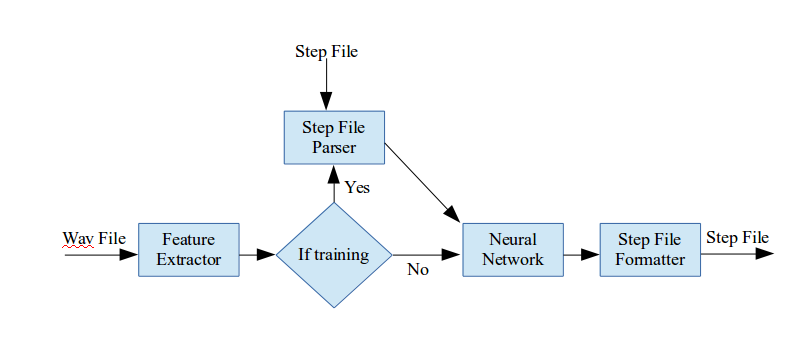
\includegraphics[scale=0.55]{data-flow.png}
\end{center}


\subsection{Feature Extraction}
Three kinds of features were used in the scope of this project. There were many other potentially useful features that could be extracted from audio files for use in beat detection, but many of them required complex audio processing beyond the knowledge of the authors of this report. This project focused on power variance, bandwidth power variance, and change in peak frequency. To accommodate for audio temporal masking in human hearing the sample rate was decreased to a sample every three milliseconds. This was done by aggregating samples into a chunk and comparing that with the other aggregated samples in its neighborhood. A chunk of data is the number of samples calculated to span three milliseconds of time.

\begin{align*}
	\text{chunk size} = c &= \frac{\text{number of samples}}{300}\\
\end{align*}

Each type of feature extraction generated data relative to the song it is in. This is due to the range of song genres considered in the scope of this project. Data comparisons using absolute values would confuse the training data when transitioning between songs, for example the electronic music has a much higher average frequency than dubstep. The solution to this was to compare features to a neighborhood of data to get relative values.

Since most songs go through various phases in which the pitch, tempo, and power levels can be drastically different the neighborhood of comparison was limited to one seconds worth of data. This value was chosen because it was small enough to capture the changes in features while still being large enough to contain data about the current state of the song. One second is also the unit used when describing the tempo of a song when making a rough estimate. This allowed for a benchmark of what would be a reasonable number of beats in a second when comparing to the genre of the song.

\subsubsection{Power Variance}
The waveform of a sound file represents its data as energy levels within a channel at a given sample. The total power level of a sample can be calculated by summing the square over all channels in the waveform.

\begin{align*}
 	\text{Power}(x) &= \sum_j^{channels} x[j]^2
 \end{align*}

Aggregation was done through averaging to lessen the number of samples being fed into the the network and to try to remove some of the noise within the signal.

\begin{align*}
	\text{Chunks}(x) &= \frac{\sum_{i=0}^{c}\text{Power}(x+i)}{c}
\end{align*}
The averaged power of a chunk is then compared to the average power of the surrounding second of data to account for different median power levels based on genre of song or mood at that moment within the song.

\begin{align*}
	\text{PowerVariance}[x] &= \text{Chunks}[x] - \frac{\sum_{i-150}^{i+150}\text{Chunks}[i]}{300}
\end{align*}

\subsubsection{Bandwidth Energy Variance}
The power level of a song ignores the frequency aspect of audio processing. The frequency of sounds within a song heavily influence the placement of beats and thus cannot be ignored. To account for this a feature was added that breaks a chunk into frequencies and sums the energy within set bandwidth ranges. These ranges were pulled from a paper written by Eric Scheirer in which he attempted to detect beats in music using only frequency analysis. In it he outlined 5 bandwidth ranges to group by, 0-200Hz, 200-400Hz, 400-800Hz, 800-1600Hz, and 1600-3200Hz\cite{bandwidthbreaks}. Frequencies over 3200Hz were ignored as their prevalence in music is limited due to discomfort caused to listeners.

First the energy across channels is calculated to account for multichannel songs.
\begin{align*}
 	\text{Energy}(x) &= \sum_j^{channels} x[j]
 \end{align*}

 The audio file is once again aggregated into chunks of roughly three milliseconds worth of data. The aggregation function is now a Discrete Fourier Transform. This was calculated using Python's SciPy library.

 \begin{align*}
 	F[i] =  \texttt{scipy.fft}(Energy[i \dots i+chunkSize])
 \end{align*}

The signals in F were divided into the above stated bandwidth ranges and their amplitudes summed. This represents the value of the cumulative power within each bandwidth range. These values were then compared to the surrounding second's worth of data using the same procedure as used when calculating the average power variance. This resulted in five values representing the power variance across the five bandwidth ranges for that chunk of data.

\subsubsection{Peak Frequency Change}
One of the biggest methods used by humans for identifying beats is to detect changes in the dominant frequency. This is used in the music genres aimed at dancing (the primary focus of this report was on such songs) to sync up crows by having frequent changes between a high pitched melody and a low pitched base line. An extreme example of this is a drop in typical dubstep songs. This feature most closely represents how humans intuitively detect beats.

The peak frequency for a chunk was found by calculating the energy for sample and taking the Fast Fourier Transform of each chunk using the same procedure as used when calculating the bandwidth energy variance. The peak frequency was found by finding the highest amplitude within the chunk in question's data and taking the frequency at which it occurred. This value itself means very little since different song genres and within the songs the median frequency varies greatly. Unlike previous features, comparing the peak frequency to the surrounding second's worth of data would make little sense since the peak frequency varies greatly within a second. Instead, the peak frequency is compared only to the next value. This aims to identify only the instance of a sudden drop to try to refine beat identification.


\subsection{Dataset Construction and Format}
\subsubsection{Dataset Format}

In order to use a multilayer perceptron network, supervised learning must be used in order to let the network learn the function you are trying to represent or approximate. For our project, the network is trained on a set of timeframes corresponding to the wavelet file for an audio track in order to detect beats. A timeframe can be defined as a portion of the audio signal for a music file. Thus, a dataset that mapped different timeframes of an audio file to a beat was required. This required researching into datasets that exposed both the metadata information for a large corpus of  audio files, and the discrete times for when beats occur.\\

With the above requirements, we could define the necessary format of our dataset. Our dataset required pairs of files for an audio track : an uncompressed wavelet file in the ‘.wav’ format and a corresponding ‘.beats’ file containing comma separated times for when beats occurred in a song.\\

\subsubsection{Music Information Retrieval Evaluation Exchange (MIREX)}

Our initial dataset was a small dataset used for a 2012 audio beat tracking competition provided by the Music Information Retrieval Evaluation Exchange (MIREX). MIREX is a contest and conference organized by the graduate school of computer science at the University of Illinois Urbana-Champaign. It provides datasets for contests attempting to identify optimal algorithms for beat detection, tempo change detection and other audio analytics. \\

The dataset used consisted of 100 songs, where each song had a file containing the times when a human audience believe beats occurred. Each audio file was in the uncompressed wavelet format, with 1 audio channel and at a standard 44.1KHz sampling rate of timeframes per second. However each song in this dataset was less than 30 seconds in length, so it did not provide enough timeframes to train any neural network model. \\

\subsubsection{Million Song Dataset}

The Million Song Dataset is a dataset containing audio analysis features for millions of songs. One of the features analyzed and available, is the discrete timing of beats. This dataset is openly available and was produced by the Echo Nost, an audio analytics company. This dataset provided all of the necessary beats information for an incredibly large corpus of songs, 280GB in size. However, unlike the Mirex dataset, it did not provide any media files that would allow us to use as training inputs to our model. Thus, we had to implement our own solution.

\subsubsection{Google Play Music}

In order to build a corpus of media files, we used the GooglePlayMusic API to to download songs. For each song we found in a subset of the MillionSongDataset, we extracted its track title, downloaded the audio file in the MPEG-2 format (mp3), and then converted it to the uncompressed wavelet format. This conversion was performed using the popular FFMPEG utility. 
\begin{center}
	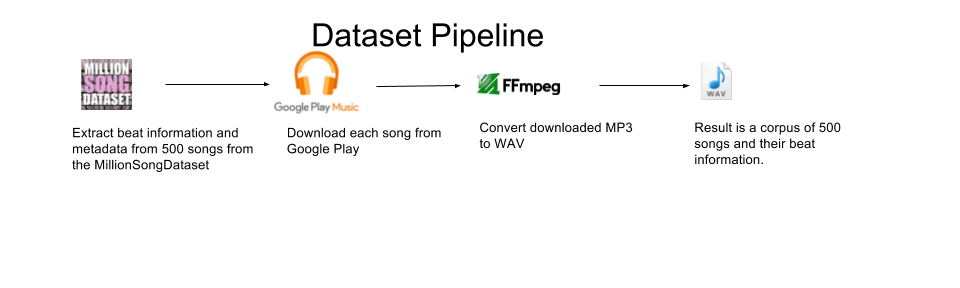
\includegraphics[scale=0.55]{dataset_flow.png}
\end{center}

\subsection{Multilayer Perceptron}
\subsection{Initial Approach}
\subsubsection{Outline}

The initial solution is to implement a simple MLP neural network which will be trained by raw input data. The intention is to observe the output of the trained network and the network itself and analyse the results to get a sense of direction.\\

\includegraphics[scale=0.55]{initial_approach_outline.png}

\subsubsection{Input Extraction}

The input of the system is pairs of files that compose a DDR game. One of the files is a music file and the other is a steps file. The DDR emulator will parse these 2 files and play the music file in sync with the steps file so the user may play the game.
The music file may come in many different formats such as MP3s, WAVs, AIFFs, and many more. However, all formats are just different representations of raw sound signals and can be readily converted to each other. Some file formats are compressed and will need to be uncompressed. The Wav file format is a standard uncompressed file format. This project converts all input music files to the Wav file format so that only one parser needs to be written. As well, the Wav file format is the easiest to work with because of its very transparent way of data storage.\\

The Wav file format [1] stores a frequency and bitrate followed by a series of sound signals that compose the sounds to be played. The frequency determines the time duration of each sound signal and the bitrate determines how many bits are used to represent each sound signal. The higher these values are, the finer the sound and the more it resembles analog sound. A parser is built to parse a wav file into memory as a list, where each item of the list will represent the amplitude of the sound signal at the time index * (1 / frequency). The wav file may contain more than one channels in which case the resulting list will have one dimension for each channel.
The steps file comes in only one file format (SM file[2]) for the PC emulator. The steps file represent the step data using measures. Each measure will contain data about which arrows will be displayed on the screen at each fraction of the measure (valid fractions are all over powers of 2). The length of each measure is specified in the header of the file, along with other various data that dictate timing factors. A parser is created to parse the steps file into memory as a list, where each item of the list will be a 1 or 0 to represent whether or not a step was present at the exact moment specified by the index. The amount of time each index represents is configurable and will be called with parameters to match that of the sound signal.\\

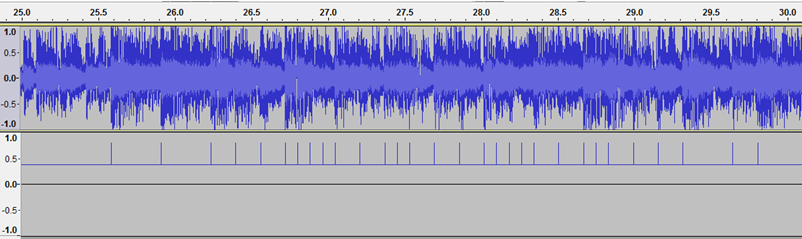
\includegraphics[scale=0.55]{signal_1.png}

Figure x. A visualisation of the sound signal array (top) and the beat signal array (bottom) of a sample input set.


\subsection{Neural Network}
A custom implemented MLP neural network is used to train the data. The configurable parameters are the number of layers, size of each layer, and the input/output size. The neural network is also able to export its current state to file so it can be imported for further training or use.\\

As mentioned previously, the input of the neural network is the raw data of the sound signal and steps signal. A series of sound signals is expected as input and a series of steps signals is expected as output. The entire signal array for both the sound and steps are split up into chunks of 100 signals, and the input/output size of the neural network is configured to 100. For a given song, one epoch consists of running each chunk of 100 signals of the song through the neural network and performing backpropagation.
The algorithm used in the MLP neural network is identical to the backpropagation algorithm discussed in lectures.\\

 At the start of each epoch, each node in the network is initialised with a random weight for each of its parent nodes. When forward propagation of data occurs, the value of the input nodes will be initialised as a chunk of 100 signals of the song. The value of other nodes is then calculated as the summation of the product of each parent node’s value and its respective weight in the current node. The value is then put through a sigmoid activation function before being used by the child nodes. The value of the output nodes is compared to the chunk of 100 signals of the steps. Error is calculated using gradient descent and back propagated. The cumulative error is calculated as the summation of (expected output – actual output) * (1 – output) * (output) across all iterations of the epoch. The weights are updated based on errors and another epoch begins. \\\\
 
 
\subsubsection{Time Analysis and Compromise}
Initial configuration of the neural network resulted in each iteration of the epoch taking around 0.00015 seconds. On average, a song will have 4 million signal samples which will result in around 40000 iterations per epoch after the subdividing the original signal into chunks. The resulting time per epoch is around 10 hours and is way less than reasonable. The parameters of the neural network were toned down to improve runtimes. The size of each layer was reduced by tenfold and so was the number of layers. This resulted in a rough improvement of 1000 times since the backpropagation algorithm was O($n^2$) on the width of the layer and O(n) on the number of layers. The resulting time per epoch was 30 seconds.\\

\subsubsection{Neural Network Training}
The neural network was trained for a single song as an initial test. The observation was that the cumulative error converged at around 1.9 after 400 epochs, from an initial cumulative error of around 400. When other songs were added to the training set, the cumulative error did not increase by a significant amount. As well, the cumulative error still converged at around 1.9. It was decided at this point that the neural network is in a trained state because the cumulative error did not improve upon further epochs. \\

\subsubsection{Results and Analysis}
The neural network implemented in this section experienced premature convergence because the cumulative error did not converge at 0. A music file was inputted into the neural network and its output was observed. The output was observed to contain values between 0.0018 and 0.0026 which meant the neural network decided that there should be no steps for the given music file. This decision was completely unwanted because it is never the case that a music file does not have a single step. As well the max and min of the output array had no observable correlation to either the expected output array or the input array.\\

With the extreme skew of the output, a different approach was used to decide the actual value of the steps output array. The output array from the neural network is used as a probability array. Each element of the array dictates the chance that a step should occur at that time. This probability is further adjusted based on the amount of time that has passed since the last step was detected. This is to account for the fact that steps will never occur too close to each other and that the distance between consecutive steps is always within some threshold.\\\\

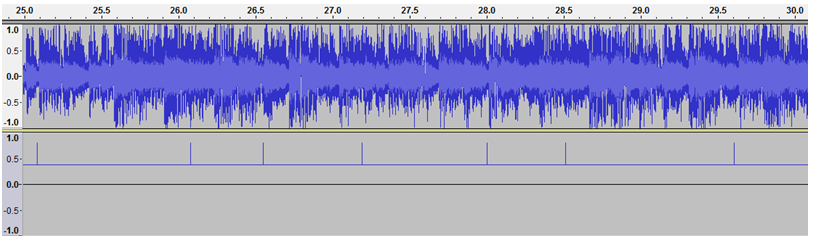
\includegraphics[scale=0.55]{signal_2.png}

Fig x. A visualisation of the input (top) and neural network output with fuzzy logic (bottom).
\\\\
The main reason for the premature convergence of the neural network is the naïve model of input and output that was used. While the sound signal array was well populated, the steps signal array was very sparse. This resulted in an expected output of 0 almost all of the time. As a result, the backpropagation algorithm will try to adjust the network so that the output is as close to 0 as possible to minimize the error. Because the 1s are so sparse, the neural network is unable to retain the learned affected weights from the 1s because they are quickly overwritten by 0s.
Another reason why the training did not go well is because of the nature of the input set. The accompanying steps file for each music file is manually generated by human beings. The human would try their best to assign steps to moments in the song where they perceive a beat or some other musical feature. However, because there is a limit to how fast a person can move their feet in a DDR game, not all beats have steps assigned to them. As a result, the steps file is somewhat of a random subset of the beats of the music file. This randomness in correlation acts to confuse the neural network during training.

\subsection{Fuzzy Logic for Input}

After analysis was done, a different way to extract input was attempted to accommodate the sparsity of the steps array. The steps parser was updated so that it may return an array of fuzzified steps. Instead of representing the precise moment of when a step occurred, a bell curve across 100 consecutive samples is used to represent the step, where the peak of the bell curve is the moment the step occurred.

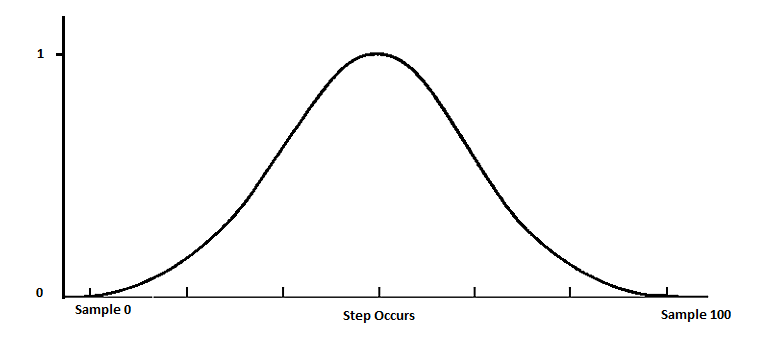
\includegraphics[scale=0.3]{fuzzy.png}

Fig x. Fuzzification of steps in steps array.
This implementation still resulted in premature convergence, with a much larger cumulative error which varies depending on the data set being used. It was conjectured that this methodology is potentially viable perhaps with a different function (instead of a bell curve) with fine-tuned parameters.\\

\subsection{Variable Learning Rate}
Another implementation was attempted to accommodate for the sparsity of the steps array. This implementation allowed the neural network to have a variable learning rate depending on the expected output of the current iteration of the epoch. If the iteration contained an expected of output of 1 in its array, the learning rate is increased to accommodate for the rarity of this expected output. This approach resulted in a trained neural net which gave output with more variance (range 0.0025- 0.0102). However, the output still did not reflect either the expected output or the input array.\\

\subsection{Summary}
The main initial approach had major shortcomings and so did its improved versions. The failures of these approaches can be easily attributed to the naivety of the assumptions made about the data. The overarching idea is that raw data is not what humans use to generate steps file or beats and that they should not be used by machines either because the goal is to simulate human steps generation. A more advanced form of feature extraction is necessary as well as possible other changes to the neural network type and parameters being used.
\pagebreak
\section{Results}
\subsection{Custom MLP Network}

\subsubsection{Time Analysis and Compromise}
Initial configuration of the neural network resulted in each iteration of the epoch taking around 0.00015 seconds. On average, a song will have 4 million signal samples which will result in around 40000 iterations per epoch after the subdividing the original signal into chunks. The resulting time per epoch is around 10 hours and is way less than reasonable. The parameters of the neural network were toned down to improve runtimes. The size of each layer was reduced by tenfold and so was the number of layers. This resulted in a rough improvement of 1000 times since the backpropagation algorithm was O($n^2$) on the width of the layer and O(n) on the number of layers. The resulting time per epoch was 30 seconds.\\

\subsubsection{Neural Network Training}
The neural network was trained for a single song as an initial test. The observation was that the cumulative error converged at around 1.9 after 400 epochs, from an initial cumulative error of around 400. When other songs were added to the training set, the cumulative error did not increase by a significant amount. As well, the cumulative error still converged at around 1.9. It was decided at this point that the neural network is in a trained state because the cumulative error did not improve upon further epochs. \\

\subsubsection{Results and Analysis}
The neural network implemented in the previous section experienced premature convergence because the cumulative error did not converge at 0. A music file was inputted into the neural network and its output was observed. The output was observed to contain values between 0.0018 and 0.0026 which meant the neural network decided that there should be no steps for the given music file. This decision was completely unwanted because it is never the case that a music file does not have a single step. As well the max and min of the output array had no observable correlation to either the expected output array or the input array.\\

With the extreme skew of the output, a different approach was used to decide the actual value of the steps output array. The output array from the neural network is used as a probability array. Each element of the array dictates the chance that a step should occur at that time. This probability is further adjusted based on the amount of time that has passed since the last step was detected. This is to account for the fact that steps will never occur too close to each other and that the distance between consecutive steps is always within some threshold.\\\\

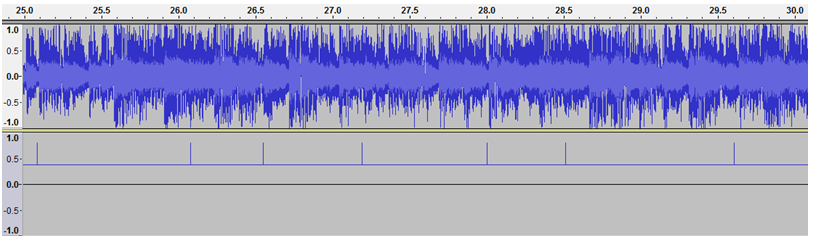
\includegraphics[scale=0.55]{signal_2.png}

Fig x. A visualisation of the input (top) and neural network output with fuzzy logic (bottom).
\\\\
The main reason for the premature convergence of the neural network is the naïve model of input and output that was used. While the sound signal array was well populated, the steps signal array was very sparse. This resulted in an expected output of 0 almost all of the time. As a result, the backpropagation algorithm will try to adjust the network so that the output is as close to 0 as possible to minimize the error. Because the 1s are so sparse, the neural network is unable to retain the learned affected weights from the 1s because they are quickly overwritten by 0s.
Another reason why the training did not go well is because of the nature of the input set. The accompanying steps file for each music file is manually generated by human beings. The human would try their best to assign steps to moments in the song where they perceive a beat or some other musical feature. However, because there is a limit to how fast a person can move their feet in a DDR game, not all beats have steps assigned to them. As a result, the steps file is somewhat of a random subset of the beats of the music file. This randomness in correlation acts to confuse the neural network during training.

\subsubsection{Fuzzy Logic for Input}

After analysis was done, a different way to extract input was attempted to accommodate the sparsity of the steps array. The steps parser was updated so that it may return an array of fuzzified steps. Instead of representing the precise moment of when a step occurred, a bell curve across 100 consecutive samples is used to represent the step, where the peak of the bell curve is the moment the step occurred.

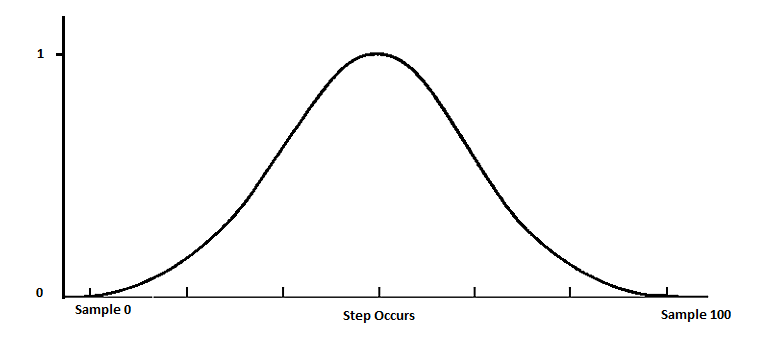
\includegraphics[scale=0.3]{fuzzy.png}

Fig x. Fuzzification of steps in steps array.
This implementation still resulted in premature convergence, with a much larger cumulative error which varies depending on the data set being used. It was conjectured that this methodology is potentially viable perhaps with a different function (instead of a bell curve) with fine-tuned parameters.\\

\subsubsection{Variable Learning Rate}
Another implementation was attempted to accommodate for the sparsity of the steps array. This implementation allowed the neural network to have a variable learning rate depending on the expected output of the current iteration of the epoch. If the iteration contained an expected of output of 1 in its array, the learning rate is increased to accommodate for the rarity of this expected output. This approach resulted in a trained neural net which gave output with more variance (range 0.0025- 0.0102). However, the output still did not reflect either the expected output or the input array.\\

\subsection{Keras MLP Network}

The results of the neural network built using Keras had inconclusive findings like our custom network. Like the custom network, this model was trained with 300 songs and each's beat information.

\subsubsection{Accuracy}

Fitting songs to the already trained model yielded accuracy $30\%$ to $60\%$. This accuracy represents the probability that a given timeframe was classified as a beat or not a beat correctly. This percentage of error  is too high for this model to be used for production systems.

\subsubsection{Error}

This model used a stochastic gradient descent algorithm with the mean-squared error function. When fitting songs to the trained model, error varied in the 0.3 to 0.7 range. 

\subsubsection{Graphs}

Using the Keras network model, we plotted the graphs indicate when our model predicted beats would occur vs. where beats actually did occur 

\includegraphics[scale=1.0]{kmp_gd.eps}

The X axis represents the timeframe at which a beat occurred. Note, these are not discrete times but sequential timeframes. The blue lines indicate when beats actually occur and the red lines indicate when the model predicted beats would occur. The Y-scale is irrelevant. Observe how the model predicts a beat for many adjacent timeframes. A correct model would have impulses for a much smaller range of timeframes, similar to how the beats actually occur.

\includegraphics[scale=1.0]{kmp_gd.png}

This graph plots the amplitude values for the given song for all of its timeframers. This is what the raw data for our model looks like when visualized. Observe that the blue and orange lines represent different channels of a wavelet file.


\subsection{Summary}
The main initial approach had major shortcomings and so did its improved versions. The failures of these approaches can be easily attributed to the naivety of the assumptions made about the data. The overarching idea is that raw data is not what humans use to generate steps file or beats and that they should not be used by machines either because the goal is to simulate human steps generation. A more advanced form of feature extraction is necessary as well as possible other changes to the neural network type and parameters being used.

\subsection{Potential Sources of Errors}

\subsubsection{Feature Extraction}
Many of the methods for extracting features from the wave file were very naive introduced approximations and rooms for error. These could have influenced more inaccuracies than a purely signal processing approach would have. It was assumed that the introduction of a neural network would compensate for weaker feature extraction.\\

The size of the neighborhood was selected using the general value of one second. This was chosen due to its unit nature and through basic reason. It should have been a tunable parameter and configured through experimentation. The neighborhood size could have greatly effected the accuracy of the data fed into the network as it was one of the primary sources of memory within the system. It is likely that one full second was far too large as it included three hundred chunks and quite a lot can happen in one second of as song, particularly one second of a dance styled song where the beats per minute are often near 140.\\

The frequencies used to break apart the bandwidths of a chunk were taken from as paper from 1998. These values were calibrated for the author's purely signal processing approach to the problem and might not have been the best for this system's approach. Other systems that more closely resemble this one have used other frequency break points determined by musical values and tones. Following one of these methods of analyzing bandwidth values would have more closely approximated the way humans hear music.\\

The sensitivity of human hearing differs greatly at different frequencies which was not considered when evaluating the way frequency interacts with how humans hear songs. The amplitude for a given frequency was its assumed ``hearablity'' value without taking into consideration the frequency itself and how that would effect how well humans would hear it. This could have been a major source of inaccuracy in the features fed into the neural network.\\


\subsubsection{Neural Network Training}
When training our two neural networks, the quantity of data used to train each was significantly less than what a real trained network would require. The beat and media files necessary were only extracted for 300 songs from the dataset we used. A neural network with many neurons like our Keras model would require many training inputs in order for backpropagation to update the weights accordingly.
\subsubsection{Neural Network Model}
The neural network models we used were simplistic in nature and not well suited to the problem. Although multilayer perceptron models can be used to classify non-linearly separable sets, other neural network models are more well suited. Specifically, models that use the concept of \textbf{memory} where previous inputs have a persistent affect on new ones, would have been useful. Such models are optimal for analyzing sequential streams of data or inputs like our audio files. Recurrent neural networks belong in this category and will be elaborated on in the conclusion.

\pagebreak
\section{Conclusion}
\subsection{Overall Results}

The findings of this report are inconclusive. Specifically, our two neural network models based on the multilayer perceptron were unable to properly predict
when beats occurred. Thus, the StepMania files generated were not correct and not human useable. The accuracy of our best models were in the 60\% although the accuracy greatly varied between songs. The loss of our error function did decrease when each model was trained but a greater dataset is required to get better results.\\

The features we extracted from audio files in order to train our model could be enhanced to be more indicative of when a beat occurs. This project used elementary digital signal processing and amplitude analysis to perform this, but more advanced techniques should exist. \\

Overall, the implementation of this project provides a system allowing a researcher to produce an audio dataset along with beat metadata for each song. This allows our work to be extensible, with the majority of future work being in the realm of building a neural network more suited to our problem. 

\subsection{Future Work, Research}

\subsubsection{Recurrent Networks}

As an alternative to regular feedforward neural networks are recurrent neural networks, where directed cycles can exist for paths through the network. Recurrent neural networks allow for the classification and regression of input vectors that are sequential in nature. Specifically, this allows the network to learn and fit input vectors, based on ones adjacent to each.\\

In the context of our problem, this fits perfectly into the audio analysis we attempt to perform. Unlike our current solution which extracts features built by analyzing adjacent timeframes for a single one, this property would be inherent to a recurrent neural network. Specifically, the concept of \textbf{memory} being in the network itself rather than encoded in input vectors would be preferable and advantageous.




\pagebreak
\bibliography{report}
\bibliographystyle{plain}



\end{document}
